%\documentclass{article}
\documentclass[10pt]{article}
\usepackage{times}
%\usepackage{natbib}
%\usepackage{multicol}
\RequirePackage{natbib}
\usepackage{amsmath, amssymb, fullpage, amsthm, array,,graphicx,asa}
%\usepackage[dvips]{graphics}

%\usepackage{hyperref} % for hyper reference

\graphicspath{{images/}}

% \usepackage{pifont} % this package is used to print check mark \checkmark
% \linespread{1.6} % factor 1.6 = double space

%\usepackage{setspace, url}
%\doublespacing



\setlength{\oddsidemargin}{0in}
\setlength{\evensidemargin}{0in}
\setlength{\textwidth}{6.5in}
\setlength{\topmargin}{-0.4in}
\setlength{\textheight}{9in}
\evensidemargin 
\oddsidemargin

\newtheorem{thm}{Theorem}[section]
\newtheorem{dfn}{Definition}[section]
\newtheorem{cor}{Corollary}[thm]
\newtheorem{con}{Conjecture}[thm]
\newtheorem{lemma}[thm]{Lemma}

%\topmargin -0.10in   % when making pdf
%\textheight 9.15in  % when making pdf

\pdfminorversion=4 % as instructed by JASA file upload


\begin{document}

% Article top matter
\title{Impact of Demographics and Skills of the Observer on Visual Statistical Inference }
\author{{Mahbubul Majumder, Heike Hofmann, Dianne Cook}
\thanks{Mahbubul Majumder is a PhD student (e-mail: mahbub72@gmail.com) , Heike Hofmann is an Associate  Professor and Dianne Cook is a Professor in the Department of Statistics and Statistical Laboratory, Iowa State University, Ames, IA 50011-1210. This research is supported in part by the National Science Foundation Grant \# DMS 1007697.}}
\date{\vspace{-.5in}}
%\date{\today}  %\today is replaced with the current date
\maketitle

\begin {abstract}  
Visual Inference is dependent on the careful evaluation of the lineups by individual observers. Each individual is different in their cognitive phycology and judiciousness which can affect the power of visual inference. To estimate the power of visual inference this can be controlled by getting evaluations from multiple people from a diverse population. But the other factor that may affect the power of visual inference is the demographics and skills of the observer. In this paper we examine this in details. The simulation experiments suggest that individual skill as well as demographics are very significant for the power of visual inference.

{\bf Keywords: \sf statistical graphics, lineup, non-parametric test, cognitive phycology, visualization, exploratory data analysis} 
\end {abstract}

%\begin{multicols}{2}
%\twocolumn

\section{Introduction} 

The fundamental concept of visual statistical inference is introduced by \citet{buja:2009} and later these concepts are validated by \citet{majumder:2012}.

\subsection{Visual Inference} A short introduction of visual inferential procedure.
\subsection{Estimation of Power of Visual Inference} Discussion of the methods for estimating the power of visual inference \citep{majumder:2012}. 

\section{Factors Affecting the Power of Visual Inference} A brief description of the factors that may affect the power of visual inference.

\subsection{Choice of Visual Test Statistic} Discuss the effective feature of visual test statistics \citep{heike:2012}. May present some results from \textit{Distance measure} of visual test statistics \citep{niladri:2012}.
\subsection{Question that Human Observer Faces}
\subsection{Observer Personality}
\subsection{Visual Perception of Human Eye} Discuss the results we have on eye tracking experiment \citep{zhao:2012}.
\subsection{Demographics of Observer}
\subsection{Skills of Observer}

\section{Simulation Experiment}

\subsection{Experiment Setup}
\subsection{Diversity of the Experimental Subjects}

\section{Results}
\subsection{Overview of the Data}
\subsection{Learning Trend of the Observer}


\begin{figure}[htbp] %  figure placement: here, top, bottom, or page
   \centering
   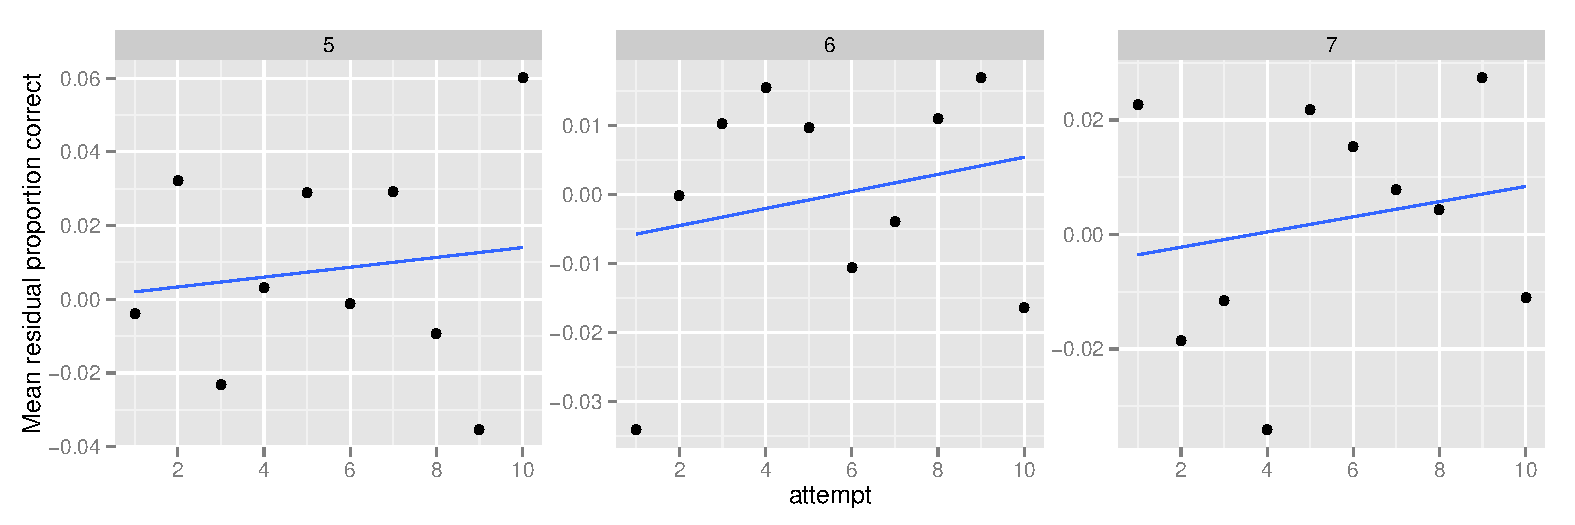
\includegraphics[width=6in]{learning_trend.pdf} 
   \caption{Probability of correct response for different attempts by each subjects for a plot with $p$-value=0.05 . The overall probability increases with attempts indicating a learning trend of the observers.}
   \label{fig:learning_trend}
\end{figure}

\section{Conclusion}


\bibliographystyle{asa}
\bibliography{references}

\end{document}



